\appendix
\chapter{自由空間伝搬損失の補償}
 ここでは,提案する信号処理アルゴリズム(図\ref{fig:System_Block_Color})の「2. transmission loss compensation」部で用いられている自由空間伝搬損失の補償の手法について述べる.

\sectuon{フリスの自由空間伝搬損}
 電波が物標に照射されると様々な方向に散乱される.この散乱の現象は物標の表面形状や粗さ,材質,入射角等の条件に大きく依存する.\\
 ここでは図\ref{fig:trans_model}に示すようなアンテナによる電波の伝送モデルを考える.ここで,送受信アンテナ間の距離$d$,送受信アンテナの利得を$G_t$,$G_r$,波長$\lambda$,そして送信電力$P_t$が与えられればフリスの伝達公式により(A.1)式のように受信電力が得られる.

\begin{figure}[H]
    \centering
    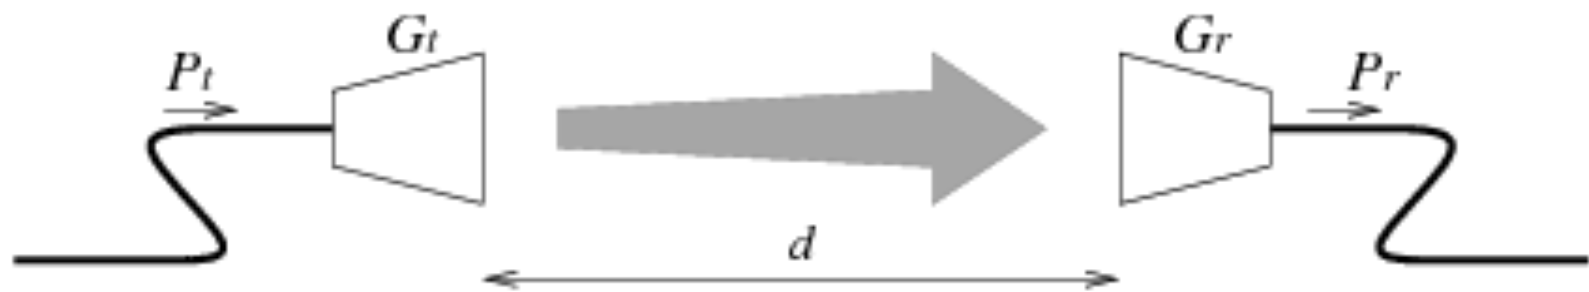
\includegraphics[width=10cm]{./fig/trans_model.png}
    \caption{電波の伝送モデル}
    \label{fig:trans_model}
\end{figure}

$$
\frac{P_r}{P_t} = G_t G_r \left(\frac{\lambda}{4 \pi d}\right)^2 = \frac{G_t G_r}{L_d}
$$

 ここで,$L_d$はフリスの自由空間伝搬損と呼ばれ,次式のように距離$d$の二乗に比例し,波長$\lambda$の二乗に反比例する.

$$
L_d = \left(\frac{4 \pi d}{\lambda}\right)^2
$$

\sectuon{補償手法}
